\documentclass[]{article}
\usepackage[margin=1in]{geometry}
\usepackage{times}
\usepackage{titlesec}
\usepackage{hyperref}
\usepackage{graphicx}
\usepackage{float}
\usepackage{amsmath}
\usepackage{booktabs}
\usepackage{caption}
\usepackage{fancyhdr}
\usepackage{multicol}
\usepackage{tcolorbox}
\usepackage{fancyvrb}
\usepackage{listings}
\usepackage{cleveref}
\usepackage{xcolor}

% --- Define the style for Python code ---
\lstdefinestyle{Python}{
    language=Python,
    basicstyle=\ttfamily\footnotesize,
    commentstyle=\color{gray},
    keywordstyle=\color{blue}\bfseries,
    stringstyle=\color{red},
    showstringspaces=false,
    tabsize=4,
    frame=single,
    captionpos=b,
    numbers=left,
    numberstyle=\tiny\color{gray},
    breaklines=true,
    title=\lstname
}

\definecolor{codebg}{RGB}{248,248,248}

\pagestyle{fancy}
\fancyhf{}
\rhead{Borrowing Strength Across Vulnerabilities}
\rfoot{\thepage}

\titleformat{\section}{\large\bfseries}{\thesection}{1em}{}
\titleformat{\subsection}{\normalsize\bfseries}{\thesubsection}{1em}{}

\hypersetup{
    pdftitle={Borrowing Strength Across Vulnerabilities: Hierarchical and Type-Aware Forecasting of Sparse Sightings},
    pdfauthor={Cédric Bonhomme, Alexandre Dulaunoy},
    pdfsubject={Forecasting vulnerability sightings under data scarcity},
    pdfkeywords={CVE, Vulnerability, Forecast, Sightings, Hierarchical model, Negative Binomial, Hurdle, CRPS, Exploitation},
    colorlinks=true, linkcolor=blue, citecolor=blue, urlcolor=blue
}

\title{\textbf{Borrowing Strength Across Vulnerabilities:\\ Hierarchical and Type-Aware Forecasting of Sparse Sightings}}
\author{
    Cédric Bonhomme \\
    \textit{Computer Incident Response Center Luxembourg} \\
    \href{mailto:cedric.bonhomme@circl.lu}{cedric.bonhomme@circl.lu} [\href{https://openpgp.circl.lu/pks/lookup?op=get\&search=0xA1CB94DE57B7A70D}{57B7 A70D}]
    \and
    Alexandre Dulaunoy \\
    \textit{Computer Incident Response Center Luxembourg} \\
    \href{mailto:alexandre.dulaunoy@circl.lu}{alexandre.dulaunoy@circl.lu} [\href{https://pgp.circl.lu/pks/lookup?op=get\&search=0x3b12dcc282fa29312f5b709a09e2cd4944e6cbcd}{44E6 CBCD}]
}
\date{2026-06-08}

\begin{document}
\maketitle

\begin{abstract}
Forecasting how often a vulnerability will be \emph{seen}---in proof-of-concept
releases, scanner detections, exploitation reports, or online discussion---is a
practical aid to defenders, but the data are notoriously hard: per CVE the series
are short (often 10--30 days), mostly zero, and punctuated by bursts. Our earlier
work \cite{bonhomme2026modeling} established \emph{qualitatively} that classical
time-series models (SARIMAX) fail in this regime and that count-based and decay
models behave more sensibly, but it could neither rank the surviving models nor
quantify the gains of any proposed improvement. This paper supplies the missing
quantitative foundation and a concrete improvement. First, we build a
reproducible evaluation harness based on proper scoring rules (CRPS, quantile
loss, RMSSE) and rolling-origin backtesting, and use it to show that a hurdle
Negative-Binomial model---which explicitly handles the over-dispersion and excess
zeros the first paper identified---is the best-calibrated single-series model,
while a time trend is actively harmful. Second, and most importantly, we attack
the root cause---per-CVE data scarcity---with \emph{hierarchical (partial)
pooling}: each CVE's activity and burst parameters are shrunk toward a population
distribution estimated from a back-catalogue of past CVEs. This dominates both
the strong rolling-mean baseline and the best unpooled model at every
training-window size and yields roughly a threefold improvement in data
efficiency; two robustness checks---a fully Bayesian treatment and a zero-inflated
likelihood---confirm that this inexpensive empirical-Bayes pooling is already
sufficient, as the binding constraint is over-dispersion rather than parameter
uncertainty or the choice of marginal count distribution. Finally, we model
sighting \emph{type}: pooling cleanly forecasts the
operationally high-value \emph{exploited} signal, although decomposing the total
by type does not help the aggregate, and---contrary to intuition---open-source
proof-of-concept and ``seen'' activity \emph{co-move} with exploitation rather
than reliably leading it. All code, data snapshots, tables, and figures are
released for reproducibility.
\end{abstract}

\vspace{1em}
\noindent\textbf{Topics:} \textit{Measuring vulnerabilities}, \textit{Forecast}, \textit{Decision}

\section{Introduction}
A vulnerability \emph{sighting} is a discrete, time-stamped observation that a
specific CVE is being referenced, discussed, or exploited---a proof-of-concept
(PoC) publication, a scanner detection template, an entry in an exploited-in-the-wild
catalogue, or a post across the Fediverse \cite{bonhomme2025scoring}. The number
of sightings a vulnerability accrues over time is a direct, observable proxy for
the attention and activity it attracts, and forecasting it---even coarsely---would
help defenders anticipate which vulnerabilities are about to matter.

In a previous study \cite{bonhomme2026modeling} we examined the feasibility of
this forecasting task and reached a largely cautionary conclusion. Sighting series
are \emph{sparse} (mostly zeros), \emph{bursty} (a PoC release or a wave of scans
produces a sudden spike), and \emph{short} (a CVE is typically only a few weeks
old when a forecast would be useful). Under these constraints, seasonal SARIMAX
models produced unstable, sometimes negative forecasts with confidence intervals
spanning orders of magnitude; count-based models (Poisson regression) and simple
decay curves were more sensible but still fragile. Crucially, that study assessed
models \emph{by eye}, from plots. This is sufficient to reject SARIMAX, but it
cannot answer the questions that matter for a deployment: \emph{Which} of the
surviving models is best? By \emph{how much}? And does a proposed refinement
genuinely help, or merely look plausible on a hand-picked example?

This paper provides the quantitative answers and a substantive methodological
advance. Our contributions are:

\begin{enumerate}
  \item \textbf{A reproducible probabilistic evaluation harness}
  (\Cref{sec:eval}) for sparse sighting forecasts, combining rolling-origin
  backtesting with strictly proper scoring rules (CRPS, quantile loss, RMSSE)
  and calibration diagnostics (interval coverage, randomised PIT). This turns the
  first paper's qualitative claims into measurements.

  \item \textbf{Count models matched to the data's pathologies}
  (\Cref{sec:models,sec:tier1}). We show that a \emph{Negative-Binomial} model
  fixes the over-dispersion the first paper observed, and that a two-part
  \emph{hurdle} addresses its excess zeros; the hurdle Negative-Binomial is the
  best-calibrated single-series model. We also show that fitting a time
  \emph{trend}---the form used previously---is actively harmful, reproducing the
  SARIMAX blow-up in count form.

  \item \textbf{Hierarchical pooling across CVEs} (\Cref{sec:pooling}), the
  central result. Rather than fitting each CVE in isolation, we treat its
  parameters as draws from a population distribution learned from past CVEs and
  shrink accordingly. This dominates every alternative at all training-window
  sizes and gives roughly a $3\times$ data-efficiency gain---directly addressing
  the scarcity that defeated the first paper. We use empirical Bayes and show, via
  two robustness checks---a fully Bayesian treatment and a zero-inflated
  likelihood---that it is sufficient: neither richer inference nor a different
  marginal count distribution improves forecasts in this over-dispersed regime.

  \item \textbf{Type-aware forecasting} (\Cref{sec:typed}), realising a stated
  goal of the first paper. Pooling the \emph{exploited} stream forecasts that
  high-value signal well; however, decomposing the total by type does not improve
  the aggregate, and a lead--lag analysis shows that PoC/``seen'' activity does
  not cleanly precede exploitation in this data---a cautionary, actionable
  finding.
\end{enumerate}

\noindent The implementation, the cached sighting corpus, and the scripts that
regenerate every table and figure in this paper are released as open source.

\section{Background and Related Work}
\paragraph{Vulnerability activity forecasting.} Most vulnerability prioritisation
relies on \emph{assessment} rather than \emph{prediction}: CVSS severity, or our
own VLAI severity model \cite{bonhomme2025vlairobertabasedmodelautomated}, which
predicts CVSS-like scores from descriptions. The Exploit Prediction Scoring System
\cite{jacobs2023enhancingvulnerabilityprioritizationdatadriven} predicts the
\emph{probability} of exploitation, and Vuln4Cast \cite{10.1145/3492328} forecasts
vulnerability \emph{publication} volumes at an aggregate level. Our task differs:
we forecast the \emph{temporal count} of observable activity for an individual
CVE. The direct predecessor of this work is \cite{bonhomme2026modeling}, whose
diagnosis (sparse, bursty, short series; SARIMAX unsuitable; count and decay
models preferable) we take as our starting point.

\paragraph{Count and intermittent-demand models.} Non-negative integer outcomes
are naturally modelled by Poisson or Negative-Binomial regression; the latter adds
a dispersion parameter for the common case where variance exceeds the mean. When
data are dominated by zeros, hurdle models \cite{mullahy1986specification} separate
the occurrence of any activity from its magnitude. The pattern of long zero runs
with occasional positive counts is precisely \emph{intermittent demand}, for which
Croston's method \cite{croston1972forecasting} and the Syntetos--Boylan
approximation \cite{syntetos2005accuracy} are the field-standard estimators; we use
them as baselines.

\paragraph{Borrowing strength.} Estimating a parameter for a data-poor unit by
shrinking it toward a population estimated from many related units is a classical
idea---Stein estimation and empirical Bayes \cite{efron1975data}, and modern
multilevel modelling \cite{gelman2007data}. Global/cross-learning forecasters such
as DeepAR \cite{salinas2020deepar} exploit the same intuition at scale. We bring
this lever to vulnerability sightings, where per-unit scarcity is the dominant
obstacle.

\paragraph{Forecast evaluation.} A probabilistic forecast should be assessed with
a strictly proper scoring rule \cite{gneiting2007strictly}; the continuous ranked
probability score (CRPS) is the natural choice and, for count data, calibration is
checked with the randomised probability integral transform
\cite{czado2009predictive}. Scaled point errors (RMSSE) as popularised by the M5
competition \cite{makridakis2022m5} allow aggregation across series of very
different magnitudes. Our harness combines these.

\section{Data and Problem Setup}\label{sec:data}
We obtain sightings from the public Vulnerability-Lookup API operated by CIRCL.
Each record carries a creation timestamp, a \texttt{type} (see
\Cref{sec:typed}), and a source. For a given CVE we aggregate records into a
gap-free daily count series, filling days with no sightings with explicit zeros so
that the calendar is regular. The forecasting target is the next $H$ daily counts
($H=7$ in all backtests; the illustrative forecasts of \Cref{sec:showcase} use a
longer 14-day horizon for readability).

\paragraph{Corpus.} To study both the data-scarce and data-rich regimes, and to
provide a credible \emph{population} for pooling, we assemble 24 CVEs: the cases
analysed in \cite{bonhomme2026modeling} plus 18 high-profile exploited
vulnerabilities (e.g.\ Log4Shell CVE-2021-44228, ProxyLogon CVE-2021-26855,
MOVEit CVE-2023-34362, Cisco IOS~XE CVE-2023-20198). Histories range from a single
11-day series (CVE-2024-9164) to nearly four years (CVE-2022-26134). \Cref{fig:data}
illustrates the regime: a rapid burst after disclosure, a heavy-tailed fade, and
long stretches of zeros---exactly the structure that frustrates smooth time-series
models.

\begin{figure}[H]
\centering
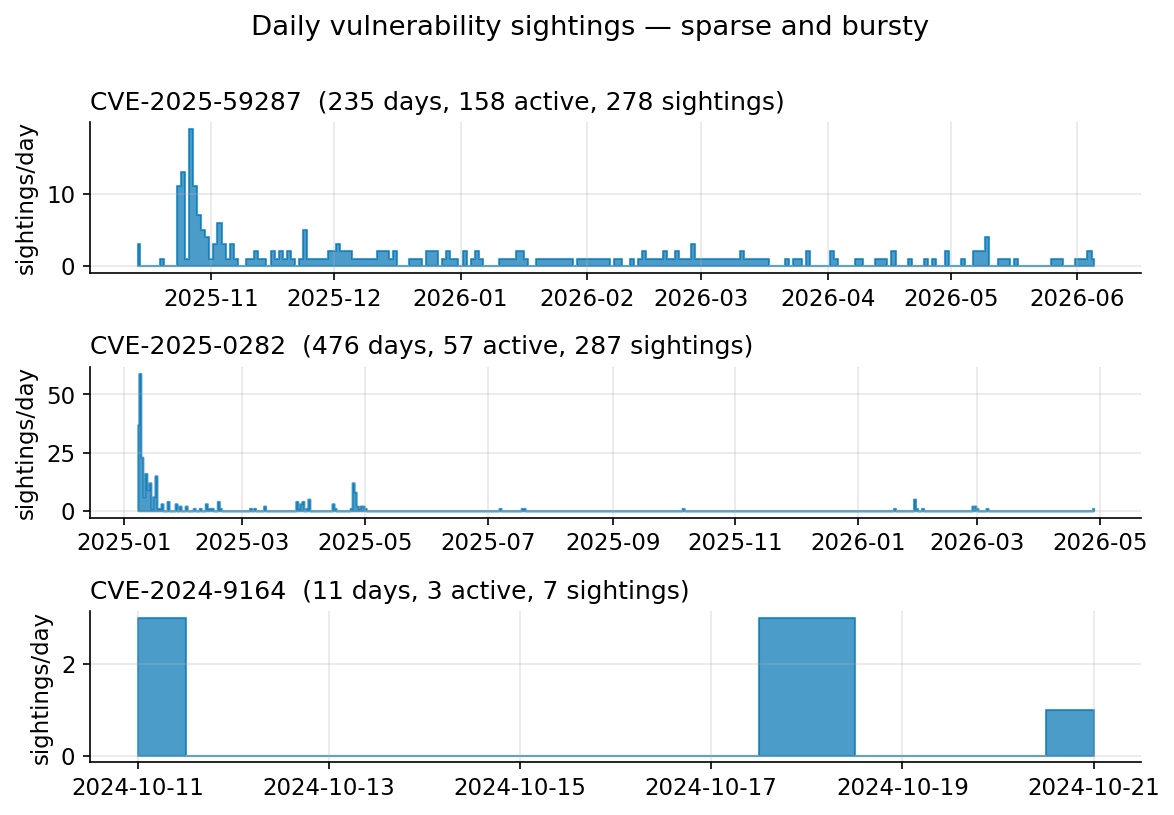
\includegraphics[width=0.85\linewidth]{figures/sightings_examples.png}
\caption{Daily sighting counts for three CVEs spanning the regime: a bursty,
fading series (top), a sharp spike followed by near-silence (middle), and an
extremely short 11-day series (bottom). Counts are low, spiky, and dominated by
zeros.}
\label{fig:data}
\end{figure}

\section{Evaluation Methodology}\label{sec:eval}
The first paper's reliance on visual inspection is the gap we close first. Three
design choices make model comparison fair and quantitative.

\paragraph{Sample-based probabilistic forecasts.} The models we compare---count
GLMs, a two-part hurdle, intermittent-demand baselines, and the hierarchical model
of \Cref{sec:pooling}---share no common closed-form predictive distribution, but
each can \emph{simulate} futures. We therefore represent every forecast as a pool
of $S$ Monte-Carlo sample paths of length $H$, and compute all metrics from those
samples. This single representation lets one scoring routine treat every model
identically.

\paragraph{Rolling-origin backtesting.} Because series are short, a single
train/test split would confound model quality with the accident of where the split
falls. We instead slide the forecast origin one day at a time; at each origin the
model is fit on the training data up to that day and scored on the next $H$ days,
so only past data is ever used and comparisons rest on a distribution of errors.
We use the protocol in two variants. \emph{Experiment~1} (\Cref{sec:tier1}) ranks
the single-series models with an \emph{expanding} window---fitting on all
observations $1{:}t$ (minimum 10 days)---over each CVE's natural history. The
pooling experiments (\Cref{sec:pooling} onward) instead use a \emph{fixed} trailing
window of $W$ days and sweep $W$, in order to probe the data-scarcity axis directly.
In both, the origin advances by one day; we draw $S=1000$ predictive sample paths
($2000$ in Experiment~1) and, to bound compute on long histories, cap the scored
origins per series at~40. The point summary, where one is needed (RMSSE), is the
predictive median.

\paragraph{Scoring rules.} For predictive samples $\{x^{(s)}_h\}_{s=1}^{S}$ and
realised count $y_h$ at horizon step $h$, we report:
\begin{itemize}
  \item \textbf{CRPS} \cite{gneiting2007strictly}, our primary metric, estimated
  from samples as
  \begin{equation}
    \mathrm{CRPS} \;=\; \frac{1}{S}\sum_{s} |x^{(s)}-y| \;-\; \frac{1}{2S^2}\sum_{s,s'} |x^{(s)}-x^{(s')}|,
  \end{equation}
  which generalises absolute error to distributions and is in the units of the
  data (sightings/day);
  \item \textbf{quantile (pinball) loss} averaged over the levels
  $\{0.1, 0.25, 0.5, 0.75, 0.9\}$;
  \item \textbf{RMSSE} \cite{makridakis2022m5}, the point error scaled by the
  in-sample one-step naive error, which is unit-free and comparable across CVEs;
  \item \textbf{interval coverage} at the 50/80/95\% levels; and
  \item \textbf{randomised PIT calibration error} \cite{czado2009predictive}: the
  mean absolute deviation of the PIT histogram from uniform, our reliable
  calibration gauge (raw coverage is inflated by structural zeros, see below).
\end{itemize}

\section{Count Models for Sightings}\label{sec:models}
\paragraph{Baselines.} A complex model must beat cheap ones to justify itself, and
RMSSE is \emph{defined} relative to a naive forecast. We include
\emph{persistence} (last value), a \emph{7-day rolling mean}, and Croston's method
with the Syntetos--Boylan correction \cite{croston1972forecasting,syntetos2005accuracy}.
Each turns a point rate into Poisson samples so it is a genuine probabilistic
forecast.

\paragraph{Poisson and Negative Binomial.} The first paper settled on Poisson
regression, which guarantees non-negative integer forecasts but imposes
$\mathrm{Var}=\mathrm{mean}$. It explicitly reported observing both over- and
under-dispersion, violating that assumption. The Negative-Binomial (NB2) model
relaxes it with a dispersion parameter $\alpha$,
\begin{equation}
  \mathrm{Var}(y) = \mu + \alpha\,\mu^2,
\end{equation}
collapsing to Poisson as $\alpha\to 0$, so it can only help at the cost of one
parameter.

\paragraph{Hurdle.} Sightings are mostly zeros with occasional bursts, and the
process that decides \emph{whether} a day is active may differ from the one that
sets \emph{how large} a burst is. A hurdle model \cite{mullahy1986specification}
makes this explicit: a Bernoulli component for $\Pr(y>0)$ and a zero-truncated
count component for the magnitude given activity. This directly targets the excess
zeros a single count model smears over.

Each count model is offered in a constant-rate (\texttt{const}) and a log-linear
time-trend (\texttt{trend}) variant, the latter matching the
\texttt{sightings\,$\sim$\,time} form used in \cite{bonhomme2026modeling}, so the
backtest can decide whether the trend earns its keep.

\section{Experiment 1: Which Single-Series Model?}\label{sec:tier1}
We backtest all models on the first paper's CVEs---five of which have enough
history for the expanding-window backtest---origin-weighted over 2296 forecasts per
model. \Cref{tab:tier1} and \Cref{fig:tier1} report the result.

\begin{table}[H]
\centering
\caption{Single-series model comparison (rolling-origin backtest, $H=7$). CRPS and
RMSSE: lower is better. PIT error: lower is better-calibrated.}
\label{tab:tier1}
\begin{tabular}{lrrr}
\toprule
model & CRPS & RMSSE & PIT cal.\ err. \\
\midrule
rolling\_mean\_7        & \textbf{0.274} & 0.298 & 0.146 \\
hurdle\_negbin          & 0.308 & 0.362 & \textbf{0.071} \\
hurdle\_poisson         & 0.321 & 0.372 & 0.105 \\
naive\_last             & 0.321 & 0.342 & 0.172 \\
negbin\_const           & 0.377 & 0.541 & 0.230 \\
poisson\_trend          & 0.426 & 0.456 & 0.180 \\
sba                     & 0.564 & 0.461 & 0.258 \\
poisson\_const          & 0.579 & 0.618 & 0.282 \\
negbin\_trend           & 4.532 & 7.641 & 0.286 \\
\bottomrule
\end{tabular}
\end{table}

\begin{figure}[H]
\centering
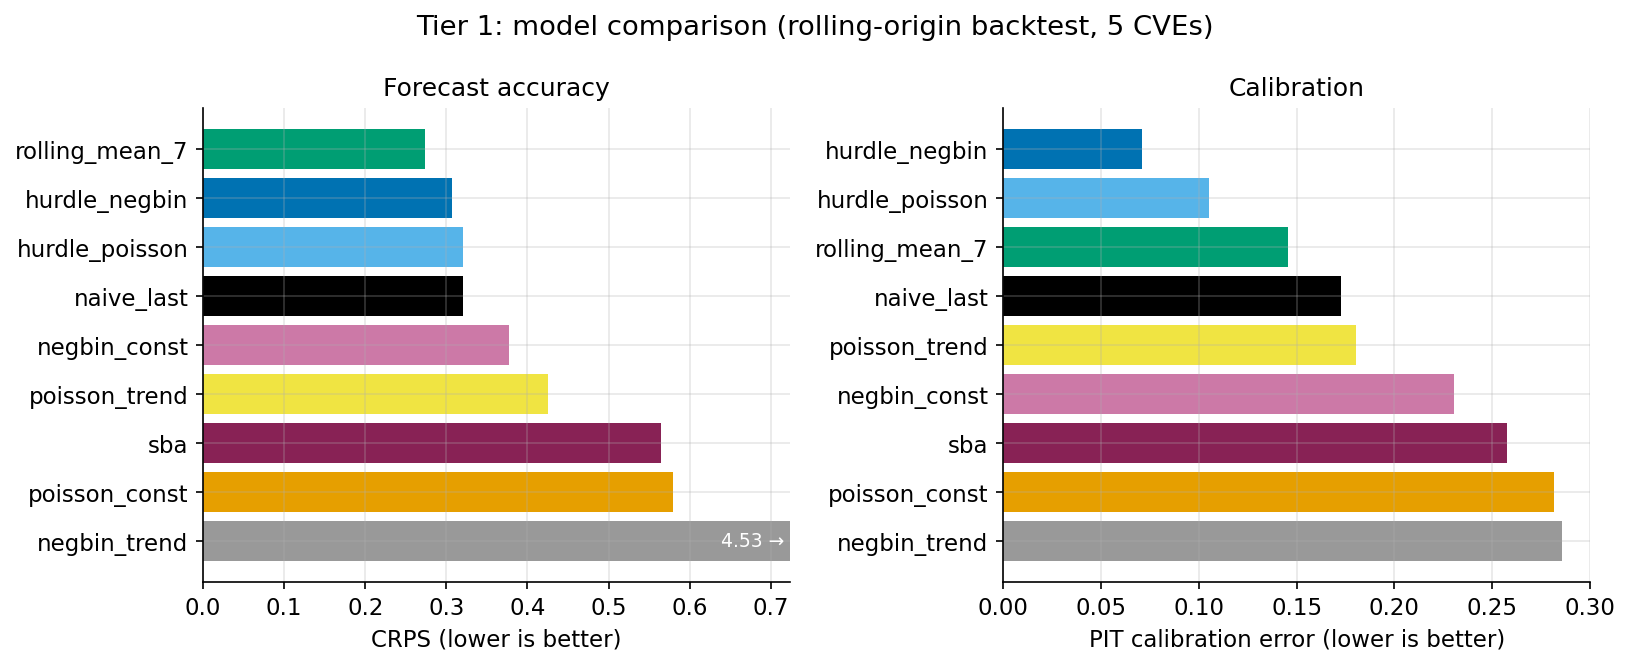
\includegraphics[width=\linewidth]{figures/tier1_model_ranking.png}
\caption{Forecast accuracy (CRPS) and calibration (PIT error) per model. The
runaway \texttt{negbin\_trend} is clipped off-axis and annotated.}
\label{fig:tier1}
\end{figure}

Four findings stand out.
\textbf{(i) Simple baselines are hard to beat}: the 7-day rolling mean has the
lowest CRPS, confirming---now by measurement---the first paper's qualitative remark
that simple averages outperform elaborate time-series models here.
\textbf{(ii) Negative Binomial beats Poisson} for the well-behaved models---the
hurdle (0.308 vs.\ 0.321) and the constant-rate GLM (0.377 vs.\ 0.579)---validating
the over-dispersion fix; the sole exception is the trend variant, where NB's
heavier tail makes the runaway extrapolation of finding~(iv) even worse.
\textbf{(iii) The hurdle Negative-Binomial is the best-calibrated model} by a wide
margin (PIT error 0.071 versus 0.282 for plain Poisson). When trustworthy
prediction intervals matter more than a marginally sharper median---the operational
case---it is the model of choice.
\textbf{(iv) The time trend is a liability}: \texttt{negbin\_trend} is the worst
model overall, because exponential extrapolation of a fitted slope reproduces the
SARIMAX blow-up in count form. Constant-rate count models are markedly more robust.
We also note that raw interval coverage over-states calibration on these series
(when the rate is low the central quantiles are both zero and the frequent zero
actuals fall inside trivially); the PIT error is the gauge we rely on.

\section{Hierarchical Pooling Across CVEs}\label{sec:pooling}
Experiment~1 improves the \emph{form} of the single-series model, but every such
model is still starved of data: with 10--30 days per CVE the activity rate and
burst size are estimated poorly. We now change the unit of learning.

\subsection{Model}
We keep the winning hurdle decomposition and assume each CVE $c$'s parameters are
draws from a shared population:
\begin{equation}
  p_c \sim \mathrm{Beta}(a,b), \qquad \lambda_c \sim \mathrm{Gamma}(\kappa,\theta),
\end{equation}
where $p_c$ is the probability a day is active and $\lambda_c$ the mean burst size
given activity. The population hyperparameters are estimated once from a
back-catalogue of past CVEs (empirical Bayes, by method of moments), and each CVE's
estimate is the conjugate posterior mean, which shrinks toward the population in
proportion to how little data the CVE has:
\begin{align}
  \hat p_c &= \frac{k_c + a}{n_c + a + b}, &
  \hat \lambda_c &= \frac{S_c + \kappa}{A_c + \theta},
\end{align}
with $k_c$ active days out of $n_c$, and $S_c$ total sightings over $A_c$ active
days. Burst sizes are sampled as $1+\mathrm{NB}(\hat\lambda_c-1)$ with a pooled
dispersion, so they are strictly positive (the hurdle assumption). A short series
starts near the population average and moves toward its own behaviour as evidence
accrues---leverage a single-series model structurally lacks. We deliberately use
empirical Bayes rather than full MCMC: it is dependency-light and instant, and
suffices to establish whether pooling helps before investing in a fully Bayesian
treatment (\Cref{sec:future}).

\subsection{Experiment: data-starvation backtest}
To isolate the effect pooling should have---helping when data is scarce---we
restrict every model to a fixed trailing window of $W$ days and sweep $W$ from 5 to
30. The population prior is estimated \emph{leave-one-out}: when forecasting CVE
$c$ it uses only the \emph{other} CVEs' full histories, mirroring the realistic
setting in which a new CVE arrives against an existing back-catalogue. We compare the
hierarchical hurdle against its unpooled counterpart---a constant-rate NB hurdle
(\texttt{indep\_hurdle\_nb}) that combines Experiment~1's two lessons, that the NB
hurdle calibrates best and that the time trend is harmful---and the rolling-mean
baseline.

\subsection{Results}
\Cref{fig:pooling} and \Cref{tab:pooling} show that the hierarchical model has the
lowest CRPS at \emph{every} window size, with the largest margin where data is
scarcest: at $W=5$ it is $\approx$25\% better than the unpooled hurdle and
$\approx$31\% better than the rolling mean. The population prior itself is
informative---mean activity 0.21, mean burst rate 2.14, pooled dispersion
$\alpha=4.52$ (strong over-dispersion, a population-level justification for NB over
Poisson).

\begin{figure}[H]
\centering
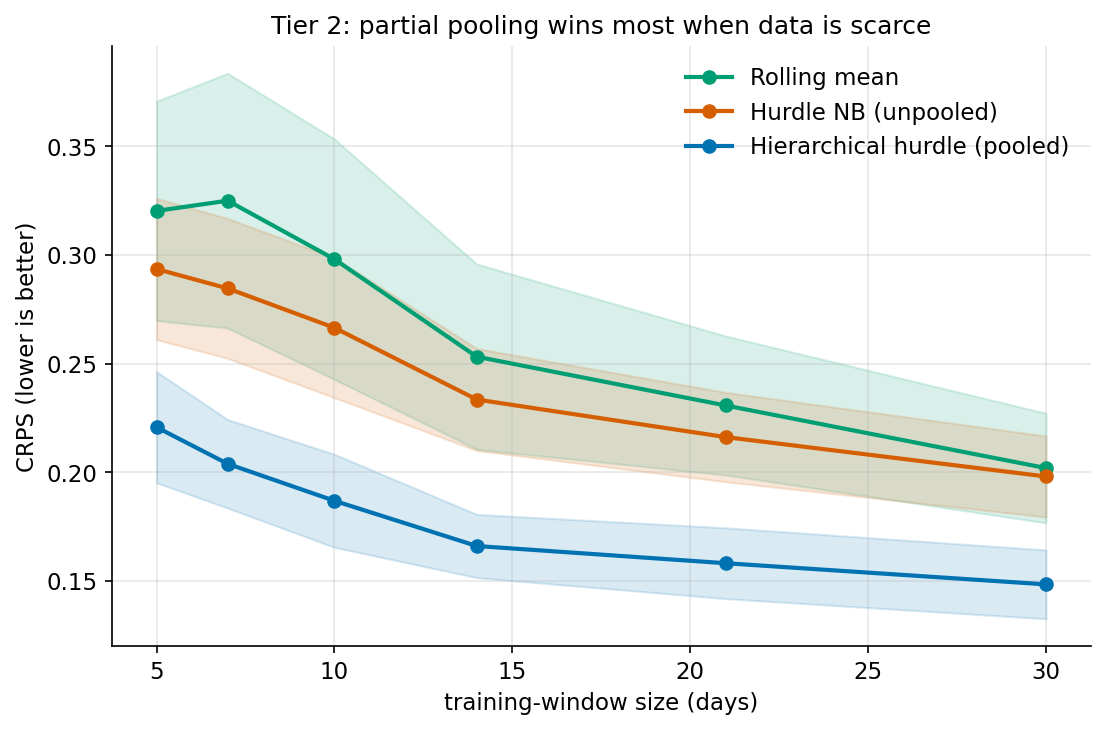
\includegraphics[width=0.8\linewidth]{figures/pooling_crps_vs_window.png}
\caption{CRPS versus training-window size (mean $\pm$ SEM). The pooled
hierarchical hurdle dominates the best unpooled model and the rolling-mean
baseline at every window, most where data is scarcest.}
\label{fig:pooling}
\end{figure}

\begin{table}[H]
\centering
\caption{CRPS by training-window size $W$ (days), 24-CVE data-starvation backtest.
Lower is better.}
\label{tab:pooling}
\begin{tabular}{lrrrrrr}
\toprule
model & $W$=5 & 7 & 10 & 14 & 21 & 30 \\
\midrule
\textbf{hier\_hurdle} (pooled)   & \textbf{0.221} & \textbf{0.204} & \textbf{0.187} & \textbf{0.166} & \textbf{0.158} & \textbf{0.148} \\
indep\_hurdle\_nb (unpooled)     & 0.293 & 0.285 & 0.266 & 0.233 & 0.216 & 0.198 \\
rolling\_mean                    & 0.320 & 0.325 & 0.298 & 0.253 & 0.231 & 0.202 \\
\bottomrule
\end{tabular}
\end{table}

A useful way to read \Cref{tab:pooling} is as \textbf{data efficiency}: the pooled
model with only 10 days of history (0.187) already beats the unpooled hurdle with
30 days (0.198), and at 7 days it nearly matches it (0.204 vs.\ 0.198). Pooling
reaches in about ten days what an isolated model does not reach in a month.
\Cref{fig:forecast} makes the mechanism concrete on a single forecast: trained on a
window ending in a burst, the pooled model shrinks its expectation toward the
population and anticipates the fade, whereas the unpooled hurdle stays high and
opens a very wide interval---the count-model echo of the first paper's exploding
confidence intervals.

\begin{figure}[H]
\centering
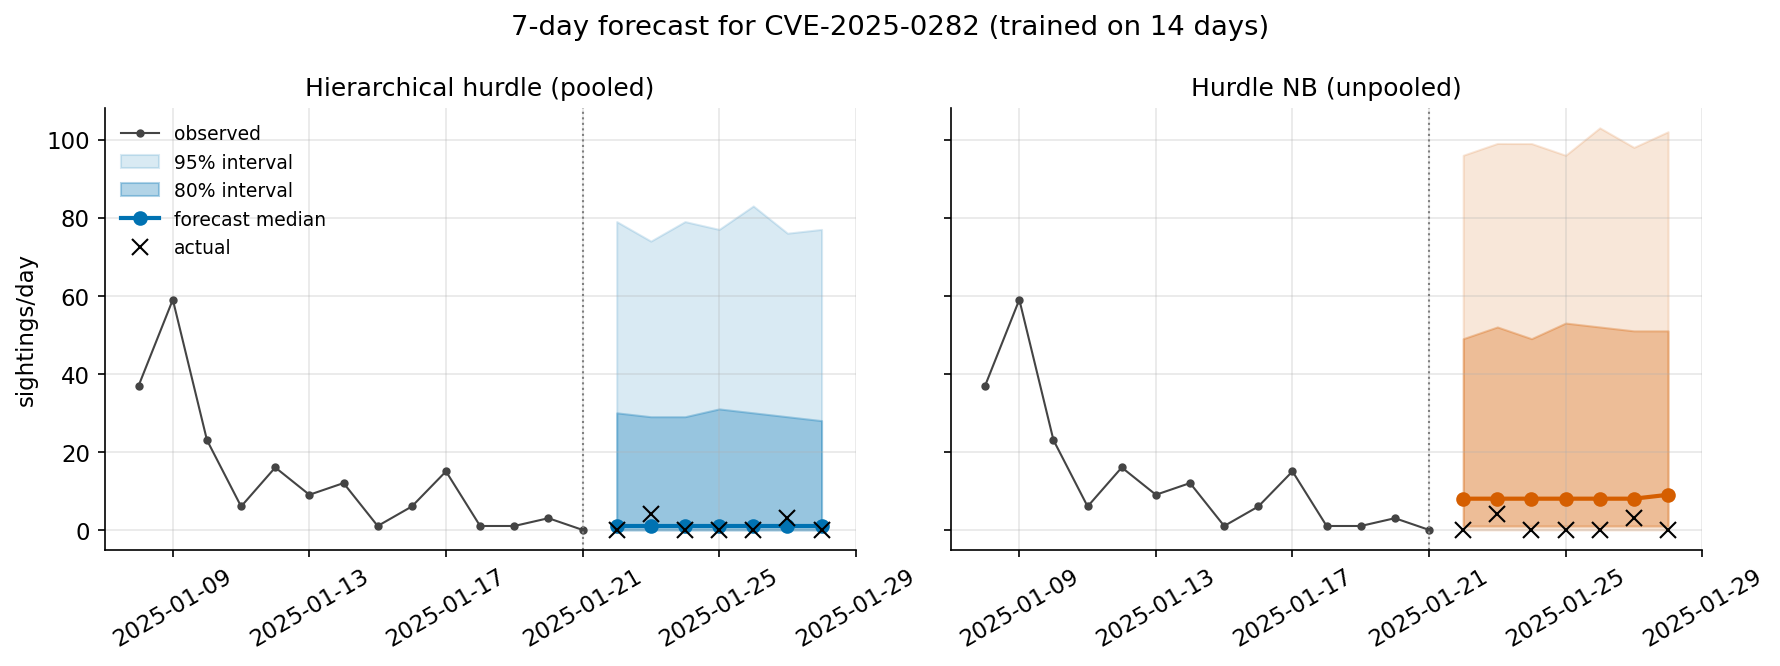
\includegraphics[width=\linewidth]{figures/forecast_example.png}
\caption{A 7-day probabilistic forecast (median, 80\% and 95\% intervals) against
realised counts, trained on a 14-day window ending in a burst. Pooled (left)
versus unpooled (right).}
\label{fig:forecast}
\end{figure}

\subsection{Does it hold at scale?}\label{sec:scale}
A 24-CVE corpus is deliberately curated, and a fair question is whether the result
survives at larger scale. We therefore repeated the data-starvation backtest on a
much larger set of \textbf{200 CVEs}---the most-sighted vulnerabilities of
2010--2026, drawn programmatically from the Vulnerability-Lookup statistics API and
spanning sixteen years and a wide range of activity profiles. The ranking is
unchanged: the pooled hierarchical hurdle has the lowest CRPS at \emph{every}
window---e.g.\ $0.127$ at $W{=}5$ and $0.098$ at $W{=}30$, versus $0.167$/$0.116$
for the unpooled hurdle and $0.176$/$0.121$ for the rolling mean (a $16$--$28\%$
reduction), and PIT calibration remains competitive. The advantage of borrowing
strength is therefore not an artefact of the small corpus; it persists, with the
same ordering, across an order of magnitude more vulnerabilities. (The eight-fold
larger corpus and its builder are released with the code.)

\subsection{Robustness: is a richer model worth it?}\label{sec:bayes}
Before accepting the empirical-Bayes hurdle, we stress-test it from two angles:
richer \emph{inference} (a fully Bayesian treatment, \Cref{sec:bayes-full}) and a
richer zero-handling \emph{likelihood} (zero-inflation, \Cref{sec:zinb}). Neither
improves on it.

\subsubsection{Full Bayesian inference}\label{sec:bayes-full}
Our pooling uses empirical Bayes: the population hyperparameters
$(a,b,\kappa,\theta)$ are point estimates. A natural concern is that ignoring
their uncertainty makes the forecasts over-confident, especially at the shortest
windows. We tested this with a \emph{fully Bayesian} variant. Conjugacy makes it
cheap and dependency-free: the per-CVE parameters integrate out in closed form
(the activity marginal is Beta--Binomial, the burst marginal Negative-Binomial),
leaving only the four hyperparameters, whose joint posterior we sample with a
short random-walk Metropolis chain in numpy/scipy---no probabilistic-programming
framework. Forecasts then propagate three layers of uncertainty: the
hyperparameter posterior, the per-CVE conjugate posterior, and count sampling.
The sampler is correct: its posterior means coincide with the empirical-Bayes
estimates (mean activity $0.220$, 95\% credible interval $0.15$--$0.30$; mean
burst rate $2.17$), now with intervals attached.

Yet the fully Bayesian forecasts are \emph{slightly worse} than empirical Bayes on
both CRPS and PIT calibration at every window (\Cref{tab:bayes,fig:bayes}). The
reason is diagnostic rather than incidental. On these zero-dominated series every
model already \emph{over-covers}---empirical 80\% interval coverage is
$\approx 0.96$ against the nominal $0.80$---so the predictive distributions are
too \emph{wide}, not too narrow. Propagating additional hyperparameter uncertainty
can only widen them further, moving coverage away from nominal and reducing
sharpness. The binding constraint in this regime is \emph{excess dispersion}, not
the parameter uncertainty that a Bayesian treatment would remedy. The inexpensive
empirical-Bayes scheme is therefore the right choice for inference; the Bayesian
machinery remains useful only where one wants calibrated credible intervals on the
population parameters themselves. This points to a complementary question---is the
\emph{likelihood} itself too loose?---which the next check addresses.

\begin{table}[H]
\centering
\caption{Empirical-Bayes vs fully Bayesian pooling vs the best unpooled model:
CRPS and PIT calibration error at selected windows. Lower is better for both.}
\label{tab:bayes}
\begin{tabular}{lrrrrrr}
\toprule
 & \multicolumn{3}{c}{CRPS} & \multicolumn{3}{c}{PIT cal.\ error} \\
\cmidrule(lr){2-4}\cmidrule(lr){5-7}
model & $W$=5 & 14 & 30 & $W$=5 & 14 & 30 \\
\midrule
\textbf{hier\_hurdle} (empirical Bayes) & \textbf{0.221} & \textbf{0.166} & \textbf{0.148} & \textbf{0.113} & \textbf{0.067} & \textbf{0.065} \\
bayes\_hurdle (full Bayesian)           & 0.229 & 0.197 & 0.167 & 0.146 & 0.089 & 0.073 \\
indep\_hurdle\_nb (unpooled)            & 0.293 & 0.233 & 0.198 & 0.093 & 0.081 & 0.105 \\
\bottomrule
\end{tabular}
\end{table}

\begin{figure}[H]
\centering
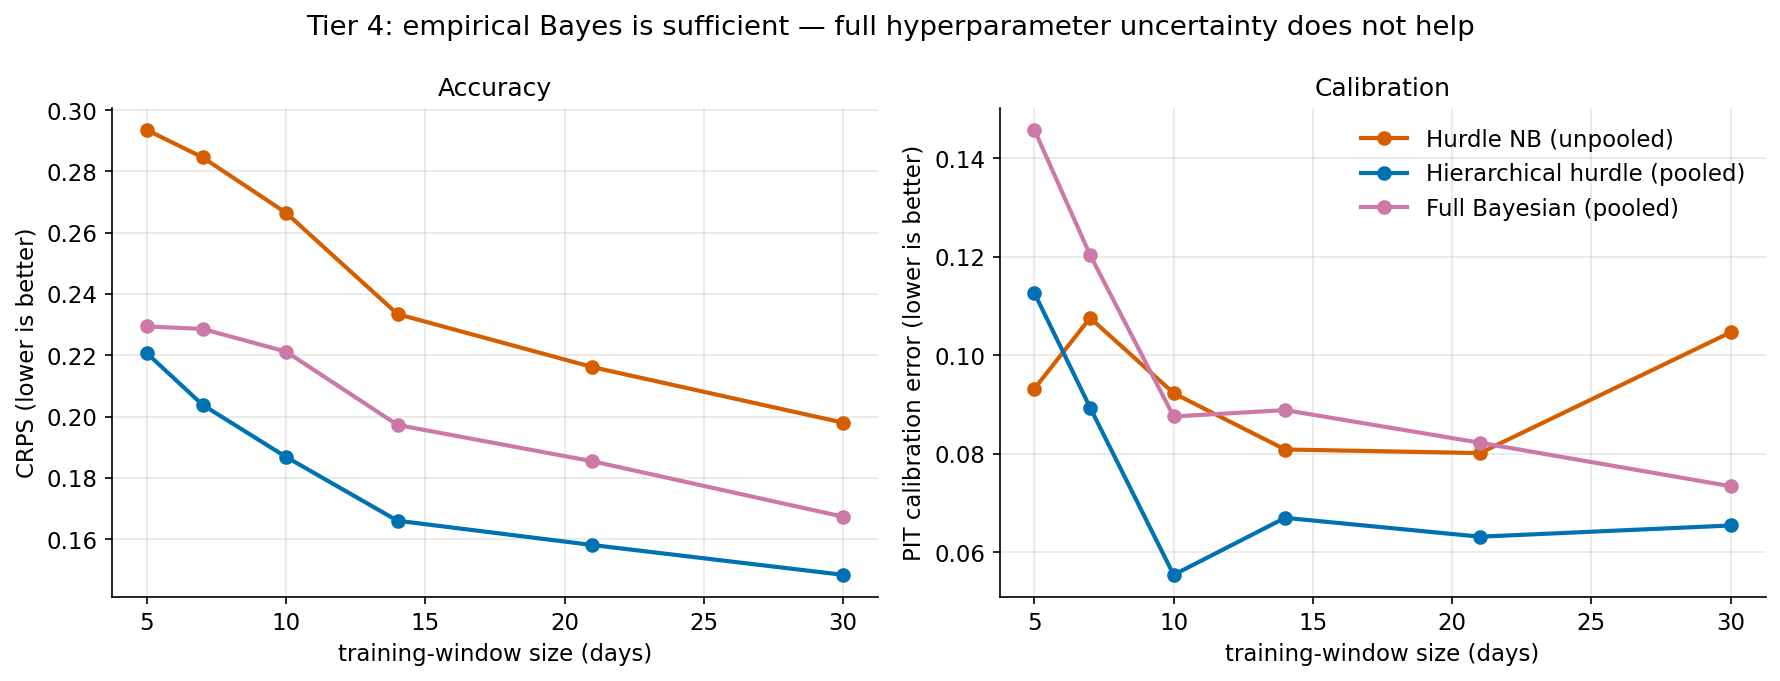
\includegraphics[width=\linewidth]{figures/bayes_calibration.png}
\caption{Accuracy (CRPS, left) and calibration (PIT error, right) versus
training-window size. The fully Bayesian model does not improve on empirical
Bayes; on this over-covering data, propagating more uncertainty hurts.}
\label{fig:bayes}
\end{figure}

\subsubsection{A zero-inflated likelihood}\label{sec:zinb}
The over-coverage just diagnosed suggests the \emph{likelihood} may be too
dispersed: the hurdle's positive part is a heavy-tailed $1+\mathrm{NB}$ with large
pooled dispersion. A zero-inflated Negative-Binomial (ZINB) is the natural
alternative---a single NB component generates the data, with an extra
structural-zero gate, so the same (potentially tighter) NB explains both the small
positive counts and some of the zeros:
\begin{equation}
  y = 0 \;\text{w.p.}\; \pi_c, \qquad y \sim \mathrm{NB2}(\mu_c, r) \;\text{w.p.}\; 1-\pi_c .
\end{equation}
We pool it identically ($\pi_c\sim\mathrm{Beta}$, $\mu_c\sim\mathrm{Gamma}$, shared
$r$). ZINB does not factorise, so we fit the per-CVE $(\pi_c,\mu_c)$ by MAP
expectation--maximisation with the population priors as pseudo-counts (again
numpy/scipy only).

The outcome separates cleanly into two observations (\Cref{tab:zinb,fig:zinb}).
\emph{Pooling still helps}: the hierarchical ZINB beats the unpooled hurdle on
CRPS at every window, so the negative result is about the likelihood, not pooling.
\emph{But the zero-inflated likelihood is worse than the hurdle}---on CRPS at every
window and, markedly, on calibration, where it is the worst of the three. Fit
honestly the ZINB count component lands at $r\approx 1$ (geometric-like, still
heavy-tailed), so it does not tighten the predictive; and where the hurdle exploits
the well-defined ``active vs.\ silent'' distinction with a hard gate on observed
activity, ZINB instead \emph{softly} attributes each zero between its two
components, which is less efficient when the zeros are genuinely structural.

\begin{table}[H]
\centering
\caption{Zero-inflated NB vs the empirical-Bayes hurdle vs the best unpooled
model: CRPS and PIT calibration error at selected windows. Lower is better.}
\label{tab:zinb}
\begin{tabular}{lrrrrrr}
\toprule
 & \multicolumn{3}{c}{CRPS} & \multicolumn{3}{c}{PIT cal.\ error} \\
\cmidrule(lr){2-4}\cmidrule(lr){5-7}
model & $W$=5 & 14 & 30 & $W$=5 & 14 & 30 \\
\midrule
\textbf{hier\_hurdle} (empirical Bayes) & \textbf{0.221} & \textbf{0.166} & \textbf{0.148} & \textbf{0.113} & \textbf{0.067} & \textbf{0.065} \\
zinb\_hier (zero-inflated)              & 0.246 & 0.208 & 0.178 & 0.146 & 0.135 & 0.161 \\
indep\_hurdle\_nb (unpooled)            & 0.293 & 0.233 & 0.198 & 0.093 & 0.081 & 0.105 \\
\bottomrule
\end{tabular}
\end{table}

\begin{figure}[H]
\centering
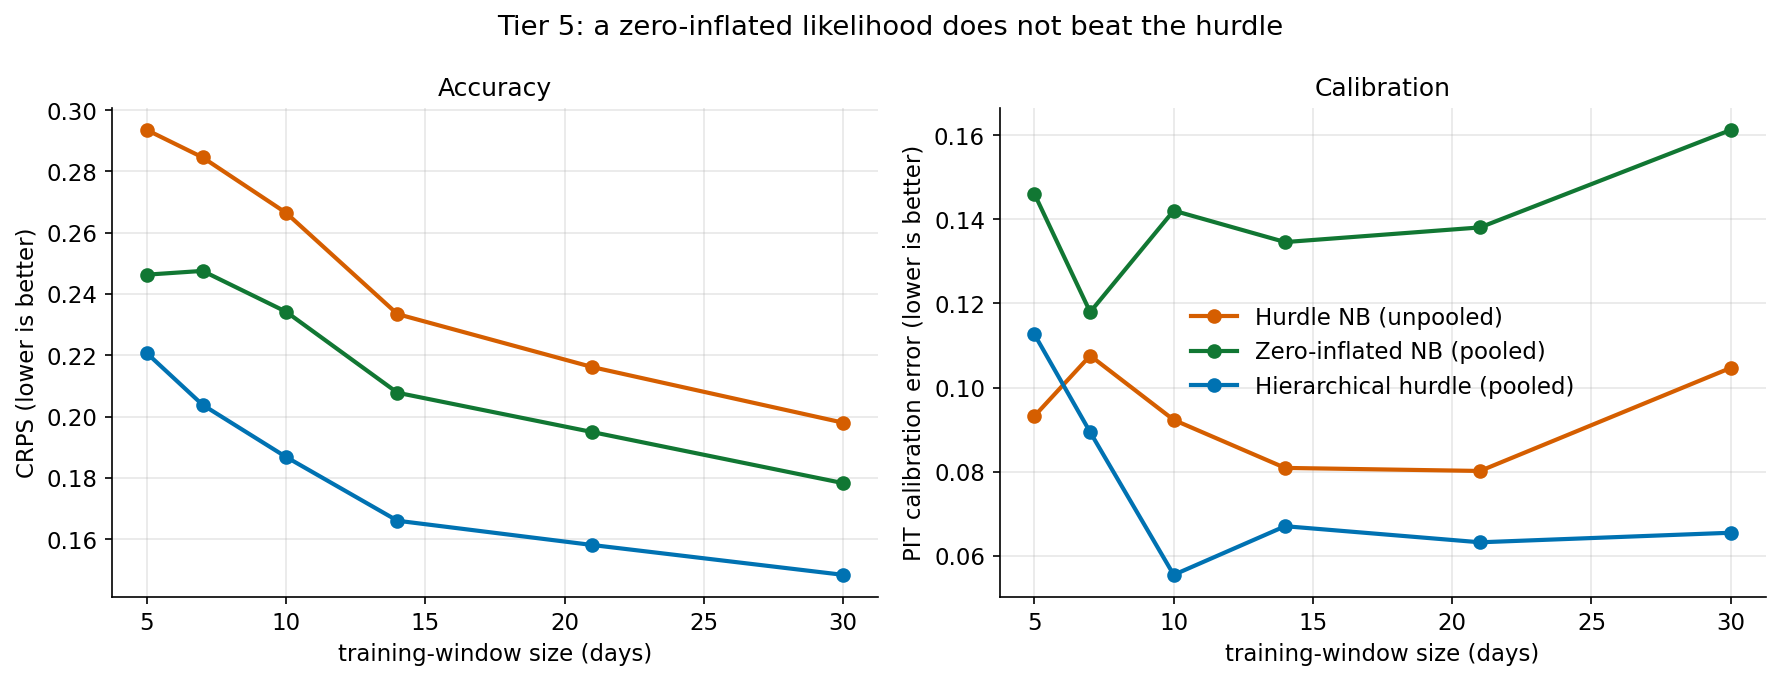
\includegraphics[width=\linewidth]{figures/zinb_comparison.png}
\caption{Accuracy (left) and calibration (right) versus training-window size. The
zero-inflated NB benefits from pooling (it beats the unpooled hurdle) but does not
beat the empirical-Bayes hurdle, and is the least calibrated of the three.}
\label{fig:zinb}
\end{figure}

\paragraph{Robustness, taken together.} Neither a fully Bayesian treatment nor a
zero-inflated likelihood improves on the empirical-Bayes hurdle. We read this as
evidence that the residual over-coverage is \emph{intrinsic} to forecasting such
sparse, bursty counts at a short horizon---a discreteness/zero effect that inflates
interval coverage regardless of the model---rather than a deficiency that richer
inference or a different marginal count distribution can remove. The empirical-Bayes
hierarchical hurdle is thus our recommended model, and the one remaining lever is to
model the \emph{dependence} the present models omit (between activity and burst, and
between sighting types; \Cref{sec:future}) rather than to elaborate the marginal.

\section{Type-Aware Forecasting}\label{sec:typed}
The first paper noted that treating all sightings as equivalent discards
information, and proposed modelling their \emph{type} to link activity to actual
exploitation. Records carry three meaningful types---\texttt{seen} (background
references), \texttt{published-proof-of-concept} (PoC), and \texttt{exploited}
(exploitation reports, largely from the CISA KEV catalogue \cite{cisakev}); two
further types are negligible ($<$0.1\%) and dropped. We pool \emph{each type
separately}, fitting one hierarchical hurdle per type with its own population
prior, and form the total as the sum of per-type forecasts.

\paragraph{Types have distinct dynamics.} \Cref{fig:typed-priors} and the per-type
priors confirm the types are not interchangeable: PoC is rare and punctual
(active on $\approx$2\% of days, low dispersion---a PoC drops once), \texttt{exploited}
is the burstiest stream (dispersion $\alpha=5.21$), and \texttt{seen} is steadier
background chatter. This heterogeneity is precisely what a single pooled total
blends away.

\begin{figure}[H]
\centering
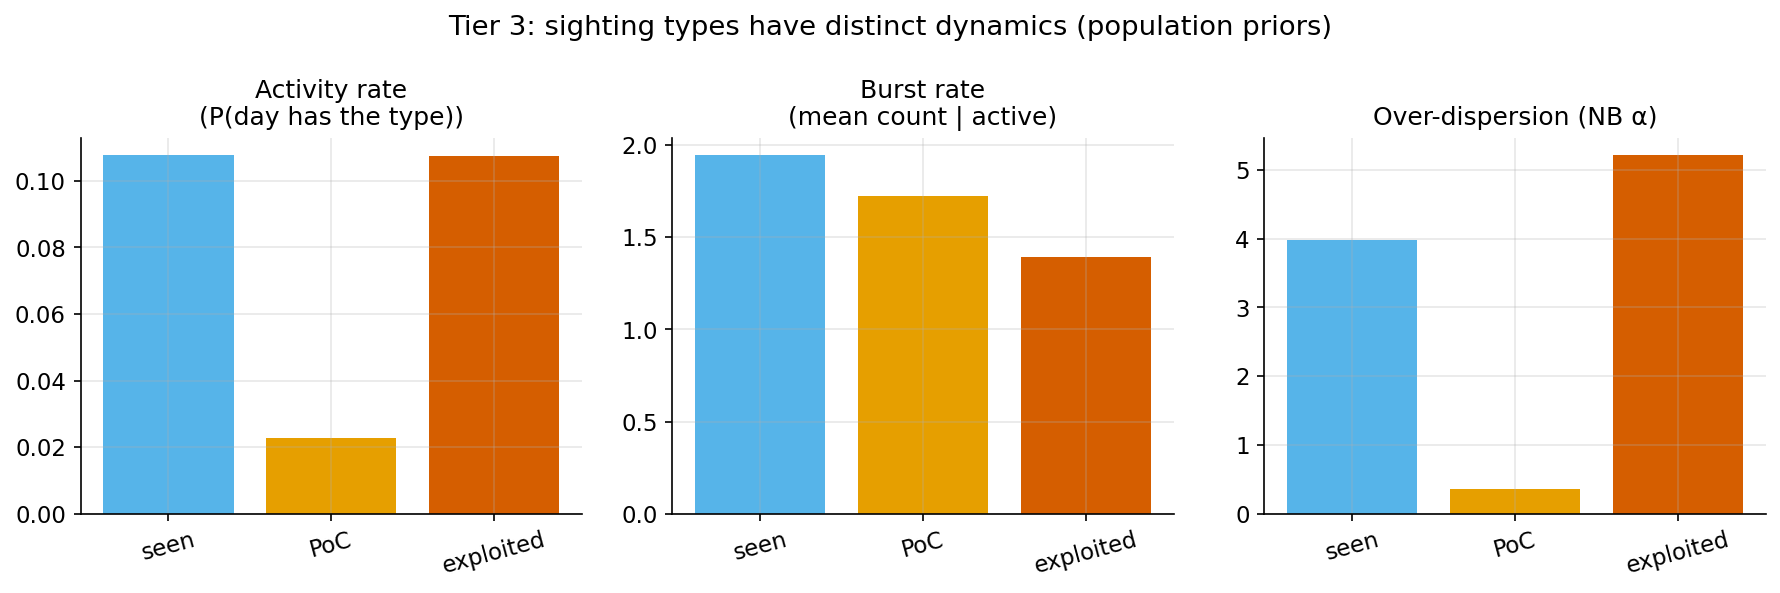
\includegraphics[width=\linewidth]{figures/typed_priors.png}
\caption{Population priors per sighting type: activity rate, mean burst size, and
over-dispersion. The types differ markedly.}
\label{fig:typed-priors}
\end{figure}

\paragraph{Pooling forecasts the exploited signal well.} The per-CVE
\texttt{exploited} stream is even scarcer than the total, so the pooling argument
should apply with more force. Repeating the data-starvation backtest on the
exploited-only series (\Cref{fig:typed-exploited}, \Cref{tab:typed-exploited}), the
type-specific pooled model again wins at every window by $\approx$25--30\% CRPS.
We can thus forecast a CVE's exploitation-related activity, with calibrated
intervals, from very little of its own history---the operationally most valuable
output.

\begin{figure}[H]
\centering
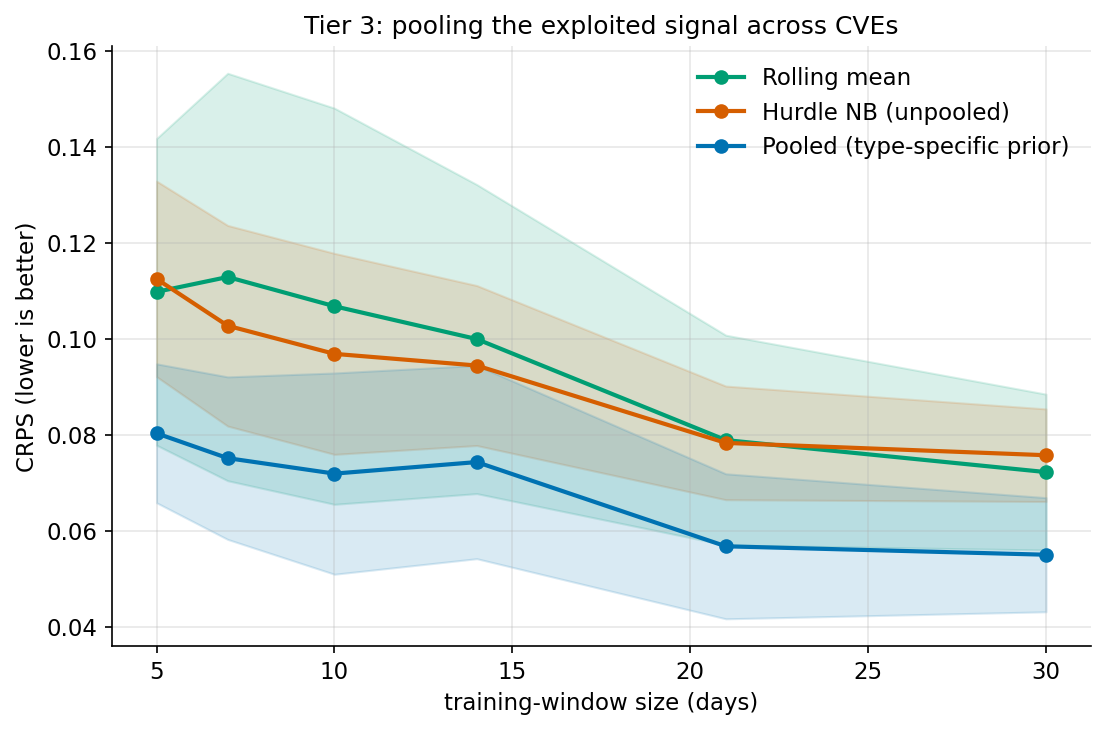
\includegraphics[width=0.8\linewidth]{figures/typed_exploited_crps.png}
\caption{CRPS on the \texttt{exploited}-only series versus training-window size.
Pooling the exploited signal across CVEs beats the unpooled hurdle and the
rolling-mean baseline throughout.}
\label{fig:typed-exploited}
\end{figure}

\begin{table}[H]
\centering
\caption{Exploited-signal CRPS by window $W$. Lower is better.}
\label{tab:typed-exploited}
\begin{tabular}{lrrrrrr}
\toprule
model & $W$=5 & 7 & 10 & 14 & 21 & 30 \\
\midrule
\textbf{hier\_exploited} (pooled) & \textbf{0.080} & \textbf{0.075} & \textbf{0.072} & \textbf{0.074} & \textbf{0.057} & \textbf{0.055} \\
indep\_hurdle\_nb (unpooled)      & 0.112 & 0.103 & 0.097 & 0.094 & 0.078 & 0.076 \\
rolling\_mean                     & 0.110 & 0.113 & 0.107 & 0.100 & 0.079 & 0.072 \\
\bottomrule
\end{tabular}
\end{table}

\paragraph{But decomposition does not help the total.} A natural hope is that
modelling types separately and summing improves the aggregate forecast. It does
not (\Cref{tab:decomp}): the single pooled total is consistently, if slightly,
better. Splitting the data across three components---and summing independent
per-type samples, which inflates variance---costs more than the per-type priors
buy back. The practical rule is therefore: \emph{use the single pooled model for
the total, and the typed model when a specific (e.g.\ exploited) forecast is
wanted.}

\begin{table}[H]
\centering
\caption{Total-count CRPS at windows 7, 14, and 30: typed decomposition versus
single pooled model.}
\label{tab:decomp}
\begin{tabular}{lrrr}
\toprule
model & $W$=7 & 14 & 30 \\
\midrule
pooled\_total (single)        & \textbf{0.203} & \textbf{0.165} & \textbf{0.148} \\
typed\_sum (decomposition)    & 0.207 & 0.177 & 0.155 \\
\bottomrule
\end{tabular}
\end{table}

\paragraph{Do PoC/seen sightings precede exploitation?} The intuitive kill-chain
suggests PoC publication should \emph{lead} exploitation. We test this with the
mean cross-correlation between each precursor type and \texttt{exploited}, over
lags $-14$ to $+14$ days (positive lag $=$ precursor leads), with each CVE's series
z-scored (\Cref{fig:leadlag}). The correlation \emph{peaks at lag 0} (seen 0.32,
PoC 0.29) and is roughly symmetric; if anything the negative lags (exploitation
leading) are slightly stronger for PoC. In this data, open-source PoC/seen activity
is therefore \emph{not} a clean leading indicator of exploitation---the dominant
relationship is contemporaneous. We attribute this largely to how
\texttt{exploited} sightings are timestamped (KEV entries are added in clusters
that need not respect the real PoC$\to$exploitation ordering), and read it as a
caution against assuming open-source chatter leads exploitation. It motivates an
event-time, first-occurrence analysis rather than daily counts (\Cref{sec:future}).

\begin{figure}[H]
\centering
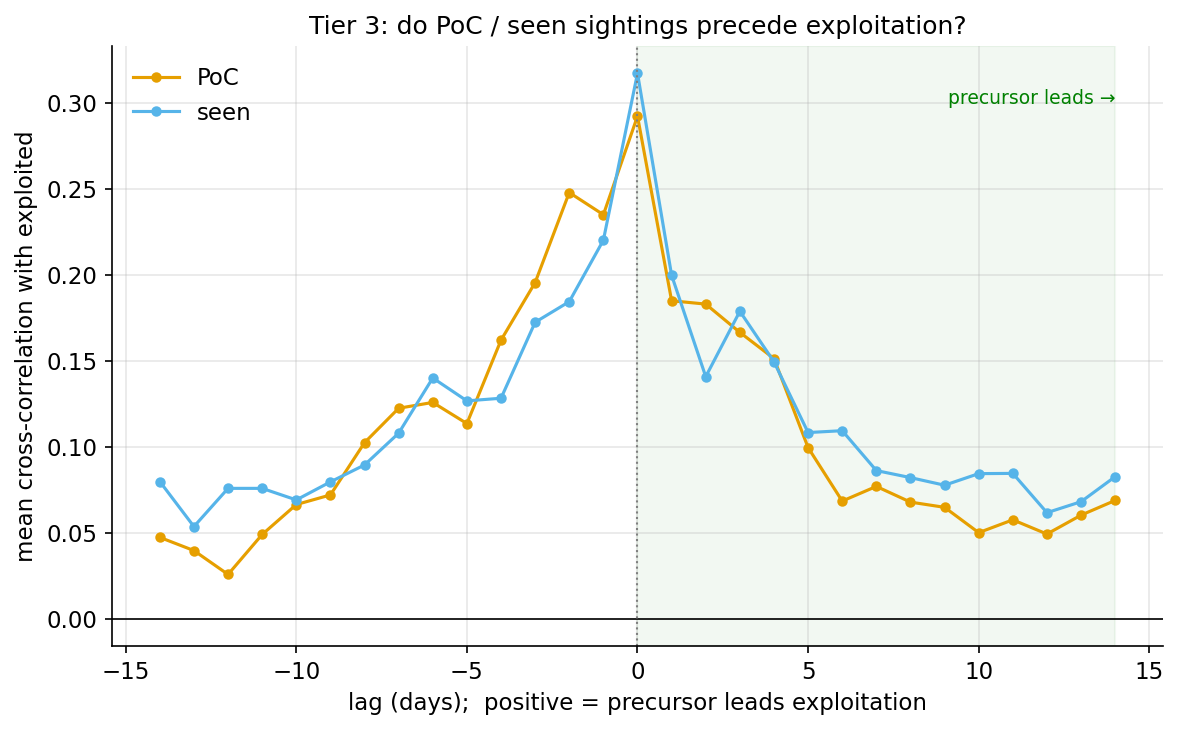
\includegraphics[width=0.8\linewidth]{figures/typed_lead_lag.png}
\caption{Mean cross-correlation of precursor types (PoC, seen) with
\texttt{exploited} activity by lag. Positive lag means the precursor leads. The
relationship peaks at lag 0 and is roughly symmetric---co-movement, not a clean
lead.}
\label{fig:leadlag}
\end{figure}

\section{Illustrative Operational Forecasts}\label{sec:showcase}
To make the recommendations concrete, \Cref{fig:showcase} shows genuine forward
forecasts for four actively-exploited vulnerabilities---Log4Shell
(CVE-2021-44228), the Cisco IOS~XE web-UI flaw (CVE-2023-20198), ConnectWise
ScreenConnect (CVE-2024-1709), and the React Server Components RCE
(CVE-2025-55182), the last under sustained rather than fading
activity---produced exactly as an operational system would.
For each CVE the population prior is fit leave-one-out from the rest of the corpus,
the recommended model is fit on the \emph{entire} observed history, and the next 14
days are forecast out-of-sample (mean and 80\%/95\% predictive intervals). The left
column uses the empirical-Bayes hierarchical hurdle on all sightings; the right
column uses the type-specific pooled hurdle on the \emph{exploited} stream alone.

Two points stand out. First, the forecasts are \emph{honest probabilistic
statements}: for these mature CVEs the expected daily count is well below one, yet
the intervals retain a realistic upper tail, reflecting that a fresh exploit
write-up or a scanning wave could reignite activity on any given day. A bare point
forecast would hide exactly this risk; the interval is the actionable output.
Second, the exploited-signal forecast (right column) is produced independently and
is the quantity a defender most cares about---isolating it, rather than reading it
off an all-sightings total, is precisely what the type-aware model of
\Cref{sec:typed} buys. These are the per-CVE forecasts a Vulnerability-Lookup
deployment could surface and refresh daily as new sightings arrive.

\begin{figure}[H]
\centering
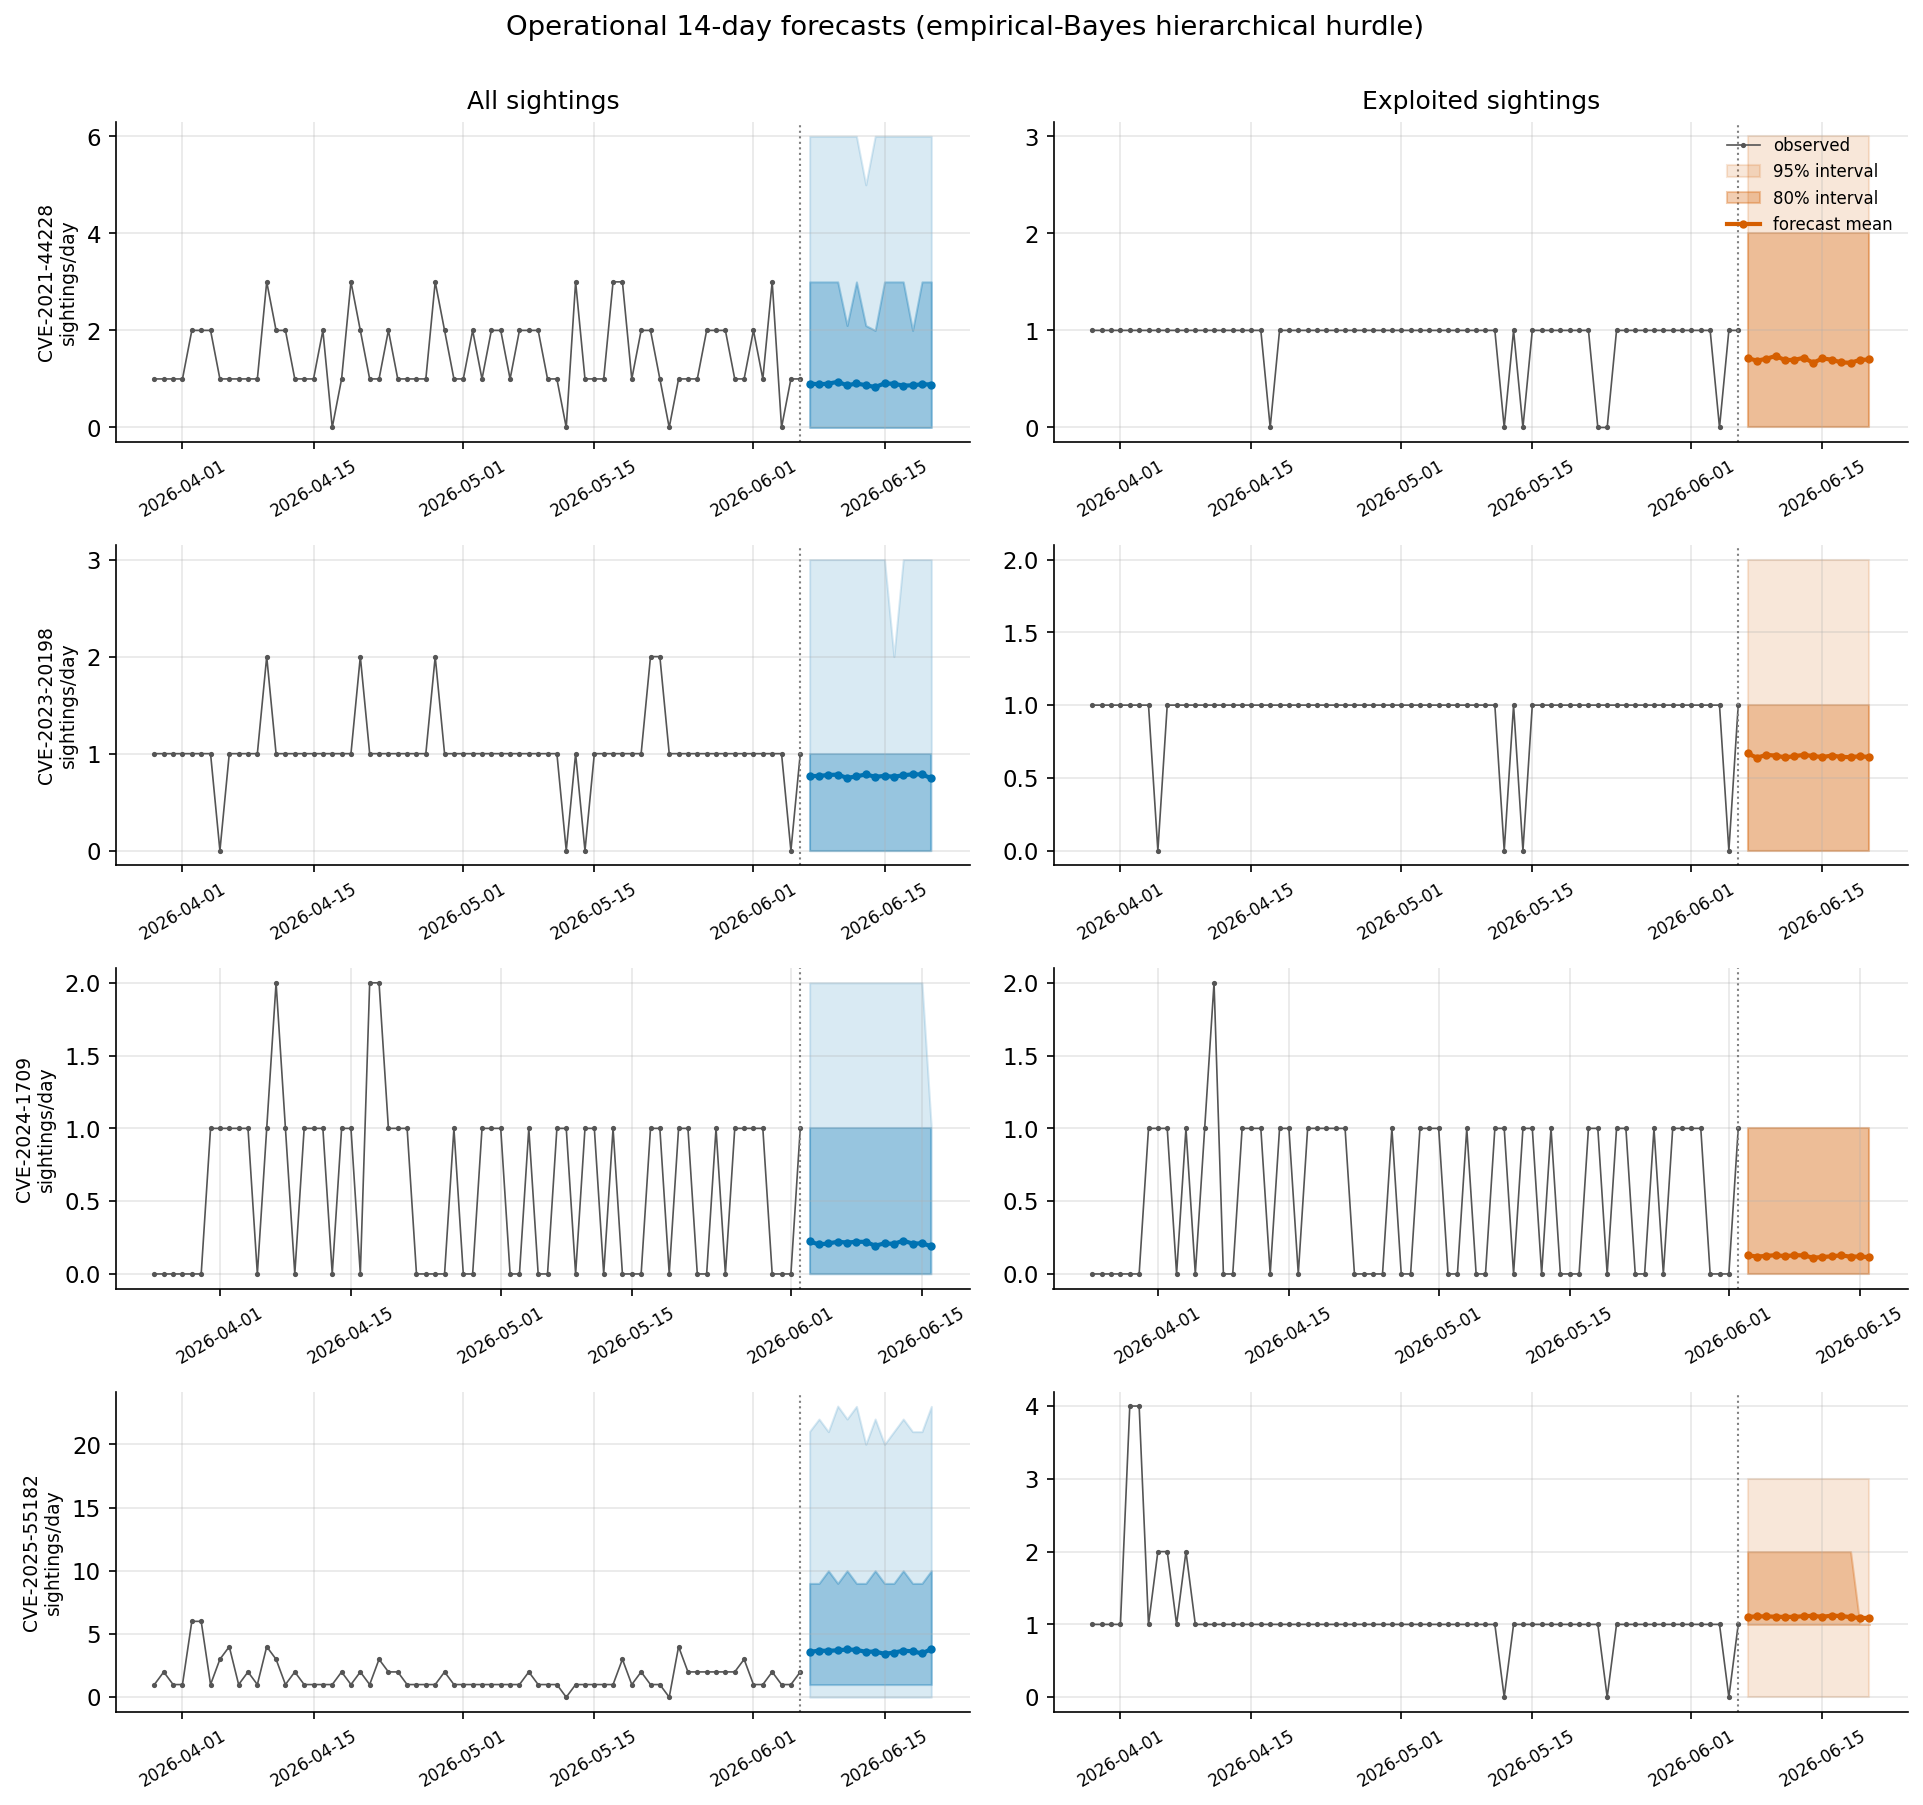
\includegraphics[width=\linewidth]{figures/forecast_showcase.png}
\caption{Out-of-sample 14-day forward forecasts for four actively-exploited CVEs,
using the paper's recommended models: the empirical-Bayes hierarchical hurdle on
all sightings (left) and the type-specific pooled hurdle on the exploited stream
(right). Grey: observed history; dotted line marks the last observation; coloured
line is the forecast mean, with 80\% and 95\% predictive intervals shaded.}
\label{fig:showcase}
\end{figure}

\paragraph{The data-scarce case.} The forecasts above use CVEs with long
histories; the regime the hierarchical model is really built for is the opposite
one---a vulnerability disclosed days ago. \Cref{fig:freshcve} shows two CVEs only
26 days old, each with an early burst already fading. Fitting a model on so little
data in isolation is exactly where the first paper's difficulties bite: the
unpooled hurdle (dashed) latches onto the recent burst and extrapolates a high,
wide forecast. The pooled model (solid, with intervals) instead shrinks toward the
population of past CVEs and projects a more measured decline---the calibrated
behaviour our backtests rewarded. This is the operational payoff of borrowing
strength: a usable, well-tempered forecast from the first weeks of a CVE's life,
when it is most needed and least supported by its own data.

\begin{figure}[H]
\centering
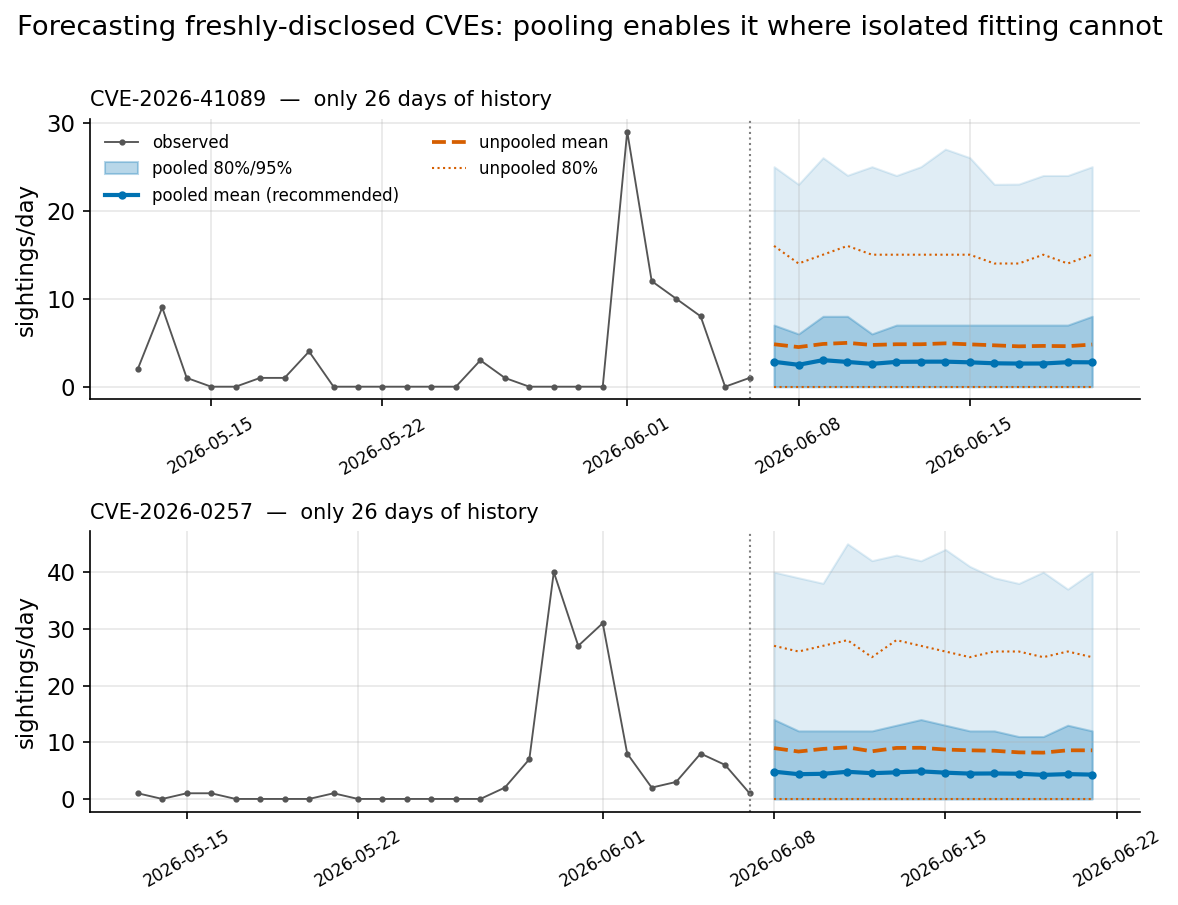
\includegraphics[width=\linewidth]{figures/short_history_forecast.png}
\caption{Forecasting freshly-disclosed CVEs (26 days of history). On so little
data the unpooled hurdle (dashed: mean and 80\% interval) over-reacts to the recent
burst; the pooled empirical-Bayes hurdle (solid, shaded 80\%/95\% intervals) shrinks
toward the population and gives a calibrated, more conservative forecast.}
\label{fig:freshcve}
\end{figure}

\section{Discussion: Operational Recommendations}
The results translate into concrete guidance for a deployment such as
Vulnerability-Lookup. (1) Adopt a probabilistic, count-based forecaster and report
intervals, not point estimates; the \emph{hurdle Negative-Binomial} gives the best
calibration among single-series models. (2) Do not fit a time trend on short
series---use constant-rate components. (3) When historical data is thin---the usual
case for a freshly disclosed CVE---\emph{pool across past CVEs}: a population prior
is the single most effective lever we found, worth roughly a threefold increase in
effective data. (4) For exploitation-relevant alerting, forecast the
\texttt{exploited} type directly with its own pooled model rather than reading it
off an all-types total. (5) Treat raw interval coverage with suspicion on sparse
counts and rely on PIT-based calibration.

These are not purely theoretical recommendations. The first paper's models are
already integrated into the production Vulnerability-Lookup instance operated by
CIRCL, and the forecaster described here---validated at the 200-CVE scale of
\Cref{sec:scale}---is being integrated into the same platform, where it will run
over the full, continuously-updated sightings stream rather than a fixed corpus.

\section{Limitations and Future Work}\label{sec:future}
Our pooled model shares a single burst dispersion rather than a per-CVE random
effect and pools the activity and burst components independently. Notably, the two
limitations one might expect to matter most do not: \Cref{sec:bayes} shows that
neither propagating hyperparameter uncertainty (a fully Bayesian treatment) nor
adopting a zero-inflated likelihood improves on the empirical-Bayes hurdle, because
the binding problem is over-dispersion intrinsic to the regime rather than
parameter uncertainty or the marginal count distribution. The clear implication is
that the remaining gains lie not in elaborating the marginal but in modelling the
\emph{dependence} the present models omit: between the activity gate and the burst
size, and---in the typed model, where the per-type streams are currently sampled
independently---between PoC and exploitation, which do co-occur.
The lead--lag analysis uses daily counts; a point-process treatment on raw
timestamps would test precedence more rigorously. Finally, time-varying covariates
with genuine variation---day-of-week effects, and EPSS
\cite{jacobs2023enhancingvulnerabilityprioritizationdatadriven} dynamics rather
than the near-constant severity score---and global cross-learning forecasters
\cite{salinas2020deepar} are promising directions our harness is now equipped to
evaluate.

\section{Conclusion}
The first study in this line concluded, qualitatively, that forecasting sparse and
bursty vulnerability sightings is hard and that classical time-series models are
ill-suited. This paper turns that diagnosis into measurement and offers a remedy.
With a proper-scoring evaluation harness we show that a hurdle Negative-Binomial is
the best-calibrated single-series model and that time trends are harmful. More
importantly, we show that the core obstacle---per-CVE data scarcity---is best
attacked not by a cleverer single-series model but by \emph{borrowing strength
across vulnerabilities}: a hierarchical model that shrinks each CVE toward a
population of past CVEs dominates all alternatives and roughly triples data
efficiency, including for the high-value exploited signal. Along the way we report
several findings that temper intuition: neither a fully Bayesian treatment nor a
zero-inflated likelihood beats the cheap empirical-Bayes pooling (the limiting
factor is over-dispersion intrinsic to the regime, not parameter uncertainty or
the marginal distribution), decomposing sightings by type does not improve the
aggregate forecast, and open-source proof-of-concept activity does not cleanly
precede exploitation in this data. Each points the same way---toward richer
\emph{dependence} structure rather than heavier machinery or a different marginal.
We release all code, data, and figures to support reproducibility and further work.

\section*{Reproducibility}
The implementation (data access, models built on statsmodels
\cite{seabold2010statsmodels}, the evaluation harness, and the scripts that
regenerate every table and figure here) is available in the TARDISsight
repository: \url{https://github.com/vulnerability-lookup/TARDISsight}.

\bibliography{mybib}{}
\bibliographystyle{plain}
\end{document}
